\documentclass[11pt]{report}
%\usepackage{fancybox}
\usepackage{geometry}
\usepackage{amsmath}
\usepackage{txfonts}
\usepackage{layout}
\usepackage{setspace}
%\usepackage{mathptmx}
\geometry{a4paper, left=22mm, right=22mm, top=25mm, bottom=25mm}
\usepackage{wrapfig}
\usepackage[dvipdfm]{graphicx,hyperref}
\usepackage{mediabb}
\setstretch{1.3}
\title{\Huge\bf{Role of Noncollective Excitations in Low-Energy Heavy-Ion Fusion Reaction
and Quasi-Elastic Scattering}}
\author{\\\\\\\\\\\\\\\\\\\\\\\\\\\\{\it\Large Department of Physics, Faculty of Science, Tohoku University}\\\\
\Huge Shusaku Yusa}
\date{March, 2013}
\begin{document}


\chapter{Random matrix theory}
In the 1960's, Wigner, Mehta, Dyson, Porter, and other people developed statistical
studies of nuclear spectra and developed a random matrix theory.
In this chapter, fundamental properties of
the random matrix theory is presented\cite{rmtrev1,rmtrev2}.

\section{Introduction}
In the 1930's, neutron cross sections are measured for heavy even-even nuclei by
using slow neutrons\cite{fermi1934, fermi1935}.
Typical experimental data are shown in Fig. \ref{resonance}\cite{BM1}.
It exhibits many narrow resonances whose width is less than 1eV and 
the energy spacing is about 20eV.
Bohr considered that these resonances
are incompatible with the independent particle
model and proposed a compound nucleus model\cite{bohr}.
Fig.\ref{compound} shows the wooden
toy model with which he described the idea of
a compound nucleus.
This figure shows the situation where a neutron is incident on the assembly of
strongly interacting nucleons.
Bohr assumed that the energy of the injected neutron
is distributed to all nucleons, and the thermal equilibrium is realized
which is the compound nucleus state.
This idea has been considered to motivate Winger to introduce the 
random matrix theory (RMT) to nuclear physics.

Afterwards, the random matrix theory is developed by Wigner, Dyson, 
Mehta, Porter and other people, whose works are compiled in Ref. \cite{porter}.
The RMT has been used to discuss the statistical properties of spectra of 
the complex strongly interacting systems.
For example, measures of the fluctuation properties of spectra such as 
the nearest neighboring spacing of levels (NNS) and $\Delta_3$ statistics can be
determined by RMT.

In RMT, instead of considering a specific Hamiltonian of a particular system,
one considers an ensemble of Hamiltonians which have the same symmetries,
assuming some probability distribution for the matrix elements.
According to the symmetries to be favored, 
there are several kinds of ensemble in RMT.
In nuclear physics, the gaussian orthogonal ensemble (GOE) is often used
corresponding to the time reversal symmetry.
Random matrix theory is applied not only to nuclear physics but also to other
fields\cite{rmtapp, MA97}. Relation to the quantum chaos is also discussed\cite{BGS84}.

\begin{figure}[t]
  \begin{center}
    \begin{minipage}[t]{75mm}
      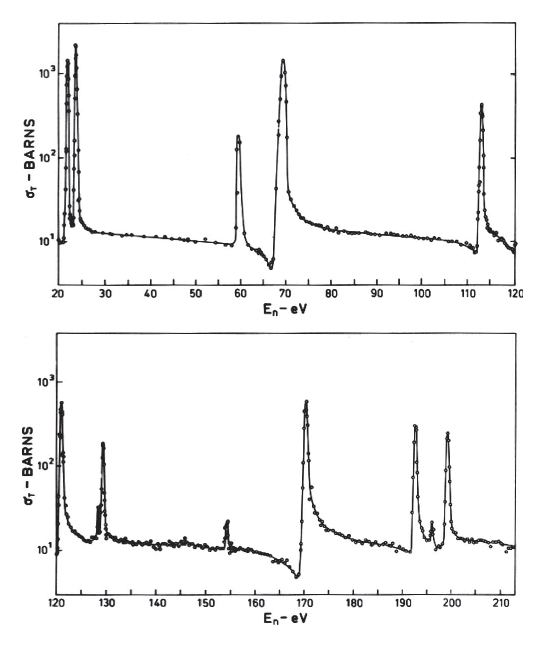
\includegraphics[clip,keepaspectratio,width=75mm]{figure/chapter4/n_res_exp.eps}
      \caption{Neutron cross sections for $^{232}$Th as a function of neutron
      energy. Taken from Ref. \cite{BM1}.}
      \label{resonance}
    \end{minipage}
    \hspace{0.5cm}
    \begin{minipage}[t]{80mm}
       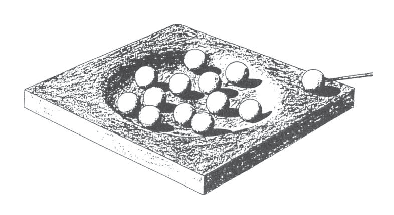
\includegraphics[clip,keepaspectratio,width=80mm]{figure/chapter4/Bohr_idea.eps}
       \caption{Bohr's Wooden toy model of compound nucleus.
       Taken from Ref. \cite{bohr}.}
       \label{compound}
    \end{minipage}
  \end{center}
\end{figure}


\section{Gaussian orthogonal ensemble(GOE)}
Hereafter, we consider assembly of levels with the same spin and the same
parity.
If a Hamiltonian is invariant under time reversal transformation,
the Hamiltonian matrix can be chosen to be real.
Thus the matrix elements satisfy
\begin{eqnarray}
H_{\mu\nu} = H_{\nu\mu} = H_{\mu\nu}^{*}.
\end{eqnarray}
The volume element in the matrix space is defined by
\begin{eqnarray}
d[H] = \prod_{\mu \le \nu}dH_{\mu\nu}.
\end{eqnarray}
By assuming that (i) there is no correlation between the matrix elements not
connected by the symmetry and (ii) the ensemble is invariant under the
orthogonal transformation, one can obtain the following probability distribution
function for the Hamiltonian matrix $H$
\begin{eqnarray}
P(H)d[H] = N_0
{\rm exp}\left\{ -
\frac{N}{4\lambda^2}{\rm Tr}(H^2)
\right\} d[H],
\end{eqnarray}
where $N_0$ is a normalization constant, $\lambda$ is a parameter, and $N$ is a
dimension of the matrix space.
If one applies the GOE to experimental data, $\lambda$ is determined from the
mean level density.
From the symmetry properties, the trace in the exponent satisfies
\begin{eqnarray}
{\rm Tr}(H^2) = \sum_{\mu,\nu}H_{\mu\nu}H_{\nu\mu}
= \sum_{\mu,\nu}H_{\mu\nu}^2 = \sum_{\mu}H_{\mu\mu}^2 +
2\sum_{\mu<\nu}H_{\mu\nu}^2
\end{eqnarray}
and the distribution function is then written as
\begin{eqnarray}
P[H]d[H] = N_0
\prod_{\mu}
{\rm exp}\left\{-
\frac{N}{4\lambda^2}H_{\mu\nu}^2 \right\}
dH_{\mu\mu}
\prod_{\rho<\sigma}
{\rm exp}\left\{ -
\frac{N}{2\lambda^2}
H_{\rho\sigma}^2 \right\}
d_{\rho\sigma}.
\label{P2}
\end{eqnarray}
From this form, one can deduce the following properties
\begin{align}
\overline{H_{\mu\nu}} &= 0 \label{eq4.6} \\
\overline{H_{\mu\nu}H_{\rho\sigma}} 
&= \frac{\lambda^2}{N}
(\delta_{\mu\rho}\delta_{\nu\sigma} 
+\delta_{\mu\sigma}\delta_{\nu\rho}) \label{eq4.7},
\end{align}
where the overline represents an ensemble average.
The first equation means that the ensemble average of the matrix element is zero,
and the second equation states that there is no correlation between 
the independent matrix elements. 
In fact, one can define GOE by a gaussian distribution function satisfying 
Eqs. (\ref{eq4.6}) and (\ref{eq4.7}),
instead of the explicit distribution function (\ref{P2}).

If one adopts the eigenvalues and eigenvectors of the Hamiltonian as
independent variables of the distribution function, Eq. (\ref{P2}) can be written as
\begin{eqnarray}
P[H]d[H] = N_0
{\rm exp}\left\{ -
\frac{N}{4\lambda^2}\sum_{\mu}E_{\mu}^2 \right\}
\prod_{\rho<\sigma} | E_{\rho} - E_{\sigma} |
\prod_{\nu} dE_{\nu}
h({\theta_i})
\prod_i d\theta_i,
\end{eqnarray}
where $E_{\mu}$ is the eigenvalues of the Hamiltonian,
$\theta_i(i=1,2,\cdots,N(N-1)/2)$ are the parameters characterizing the
eigenvectors and,
$h({\theta}_i)$ is a function only of $\theta_i$.
One can see that the distribution function is written as the product of two
parts which respectively depend only on the eigenvalues and the eigenvectors, 
that is,
the eigenvalues and eigenvectors are uncorrelated independent variables.
The factor $\displaystyle \prod_{\rho<\sigma}|{E_\rho - E_\sigma}|$
in this expression represents a level repulsion.

\section{Properties of GOE}
In this section, we review on the fundamental properties of GOE, that is,
universality and ergodicity.
First, we consider the mean level density in GOE.
It is given by
\begin{eqnarray}
\rho(E) = \overline{\sum_{\mu}\delta(E - E_{\mu})},
\end{eqnarray}
which behaves as
\begin{eqnarray}
  \rho(E) =
  \left\{
    \begin{array}{l}
      \displaystyle
      \frac{N}{\pi\lambda}\sqrt{1-\left(\frac{E}{2\lambda}\right)^2}
      \ \ \ {\rm for}\ \ \ |E| \le 2\lambda \\
      0\ \ \ {\rm for}\ \ \ |E| > 2\lambda
    \end{array}
  \right.
\end{eqnarray}
in the limit of $N \rightarrow \infty$.
This is a half circle and this behavior is called the Wigner's half circle law.
Since the actual nuclear level density exponentially increases according to the
excitation energy, this behavior is not a physical one.
However, this fact is not a problem because in using GOE, we are not interested
in the global properties of the spectrum but in the local properties like the
distribution of level spacing.
Local property means the property in the energy scale which can be ignored
compared to $4\lambda$ (diameter of the half circle)
in the limit of $N \rightarrow \infty$.
In this energy scale, the fluctuation properties of the spectrum is universal.
That is, even if the ensemble does not have a gaussian functional form but has
another cutoff, the local fluctuation measures are the same as
that of GOE as long as the
ensemble is orthogonally invariant and the spectrum appears in a finite range,
while the overall shape of the spectrum is different.
Thus, in the limit of $N \rightarrow \infty$, the local fluctuation measures are
separated from global properties of the spectrum and are universal\cite{HW95}.

Next we discuss about ergodicity. 
In GOE, the fluctuation measures are obtained by taking an ensemble average of
certain quantities. 
However, one may wonder whether it is meaningful to compare such 
quantities with the data obtained from physical system which is governed by
a specific Hamiltonian.
The ergodicity of GOE gives an answer to this question.
Experimentally obtained spectral data can be used for the calculation of 
quantities such as the distribution of nearest neighbouring spacing by averaging
over the spectrum. We denote an average of a quantity $O$ over the spectrum by
$\langle O \rangle$.
If $\overline{O} = \langle O \rangle$ holds
for all members of the ensemble and for all quantities $O$ describing local
fluctuation, one can meaningfully compare the results from GOE and the data.
Although this relation has not been proved, a weaker claim
\begin{eqnarray}
\overline{(\overline{O} - \langle O \rangle)^2} = 0
\end{eqnarray}
has been proved, that is, for almost all members of the ensemble, an averages of
$O$ over the ensemble and that over the spectrum are the same.
This property is call ergodicity.

\section{Fluctuation measures of GOE}
We introduce three famous fluctuation measures of GOE.
\begin{figure}[t]
  \begin{center}
    \begin{minipage}[t]{80mm}
      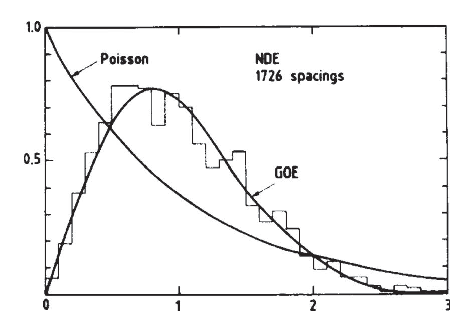
\includegraphics[clip,keepaspectratio,width=80mm]{figure/chapter4/GOEvsNDE.eps}
      \caption{Comparison of NNS distribution for GOE and
      Nuclear Data Ensemble (NDE). 
      Taken from Ref. \cite{NDE1}. A Poisson distribution is also shown.}
      \label{fig4.3}
    \end{minipage}
    \hspace{0.8cm}
    \begin{minipage}[t]{69mm}
       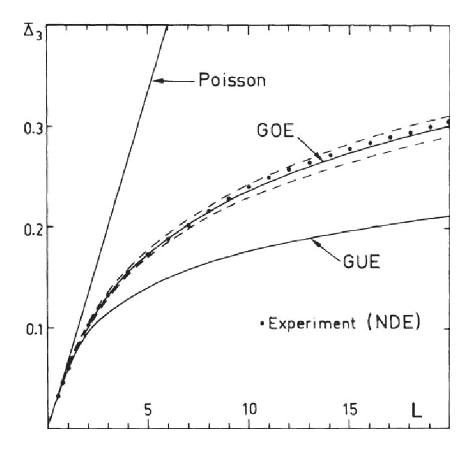
\includegraphics[clip,keepaspectratio,width=69mm]{figure/chapter4/GOEvsNDE2.eps}
       \caption{Comparison of $\Delta_3$ statistics for GOE and NDE.
                The $\Delta_3$ statistics for GUE 
                (Gaussian Unitary ensemble) and 
                Poisson distribution are also shown. Taken from Ref. \cite{NDE2}.}
       \label{fig4.4}
    \end{minipage}
  \end{center}
\end{figure}
At first, we introduce the distribution of nearest 
neighbouring spacing (NNS) of
levels. Although the distribution function cannot be written in a closed form, 
it is nicely approximated by a Wigner distribution
\begin{eqnarray}
P(s) = \frac{\pi}{2}se^{-\frac{\pi}{4}s^2},
\end{eqnarray}
where, the parameter $s$ is the level spacing divided
by the mean level spacing.
For small $s$, $P(s)$ is proportional to $s$, and this indicates a level
repulsion. If there is no correlation among levels, the distribution is given
by a Poisson distribution which has a peak at $s=0$. The level repulsion of GOE
represents strong correlation among levels.
In Fig.\ref{fig4.3}, we show the comparison of NNS distribution from
GOE and experimental data.
The data is obtained by compiling the data from neutron resonances and proton
resonances, and is called Nuclear Data Ensemble (NDE)\cite{NDE1}.
A Poisson distribution is also shown. One can see that the distribution of GOE
reproduces that of NDE well.

Next we introduce the $\Delta_3$ statistics which represents the correlation of
level spacing.
We define the following function
\begin{eqnarray}
N(E) = \int^E_{-\infty}dE^\prime
\sum_{\mu}\delta(E^\prime - E_{\mu}).
\end{eqnarray}
This represents a number of levels below the energy $E$. Using $N(E)$,
the $\Delta_3$ statistics is defined by
\begin{eqnarray}
  \Delta_3(L) = \min_{a,b}\frac{1}{L}\left\langle
       \int^{E_0+L}_{E_0}dE^{\prime}\overline{
       \left[N(E^{\prime})-a-bE^{\prime}\right]^2} \right\rangle,
\end{eqnarray}
where, $\langle\rangle$ represents an average with respect to $E_0$.
$\Delta_3(E)$ behaves logarithmic increase for large $L$
\begin{eqnarray}
\Delta_3(E) \approx \frac{1}{\pi^2}\left({\rm ln}L - 0.0678\right).
\end{eqnarray}
Comparison of this quantity from GOE and NDE is given in Fig.\ref{fig4.4}.
In the figure, the $\Delta_3$ statistics from
the gaussian unitary ensemble (GUE) and
the Poisson distribution are also shown. One can see that the GOE reproduces the
data.

Finally, we introduce a Porter-Thomas distribution which corresponds to the
distribution of eigenvectors.
Let $\psi$ be the projection of an eigenvector of a Hamiltonian in GOE 
on to some axis in Hilbert space.
The quantity $y = \psi^2/\overline{\psi^2}$ obeys the,
Porter-Thomas distribution given by
\begin{eqnarray}
P(y) = \frac{1}{\sqrt{2\pi y}}e^{-\frac{y}{2}}.
\end{eqnarray}
This distribution is compared with, for instance, the transition probability to
a final state of nuclear levels or the width of the decay to a final state,
because these quantities are proportional to the absolute square of the matrix
elements containing the wave function.





\section{Random matrix theory for deep inelastic collision}
In the previous sections, we have reviewed general aspects of
RMT. In this section, we review the application of RMT to deep inelastic
collision by Agassi, Ko, and Weidenm\"uller
in the 1970's\cite{KPW76, AKW78, BSW78, akw1,akw2,akw3,akw4}.
A similar model is employed in Ref. \cite{BDK96} for the study of dissipation in
collective motion of a quantum many-body system.

In the 1970's, heavy-ion reactions in the energy region of
a few million electron
volt per nucleon had revealed a new form of reaction not classified either
to a direct reaction or to a compound nucleus reaction.
It exhibits large dissipation of
the kinetic energy into the energy of intrinsic excitations and is called deep inelastic
collision (DIC). Classical models employing a
friction force has been used for the description of DIC.
Weidenm\"uller and his
collaborators developed a random matrix model aiming to describe DIC in a more
microscopic point of view.
They took advantage of the complex nature of the highly excited states relevant
to DIC, that is, they imposed a statistical random matrix assumption for the coupling matrix 
which couples the relative motion and the intrinsic excitations.
Based on RMT, they assumed the following condition
for the second moment of the coupling matrix
elements between the intrinsic states $|nIM\rangle$
\begin{align}
&\overline{
\langle nIM| V_{\rm coup}(\bvec{r}) |n^\prime I^\prime M^\prime \rangle
\langle n^{\prime\prime}I^{\prime\prime}M^{\prime\prime} |
        V_{\rm coup}(\bvec{r^\prime}) 
        |n^{\prime\prime\prime}I^{\prime\prime\prime}M^{\prime\prime\prime}
\rangle} \nonumber\\
=& 
\left\{\delta_{nn^{\prime\prime}}\delta_{n^{\prime}n^{\prime\prime\prime}} 
       \delta_{II^{\prime\prime}}\delta_{I^{\prime}I^{\prime\prime\prime}}
   +   \delta_{nn^{\prime\prime\prime}}\delta_{n^{\prime}{n^{\prime\prime}}}
       \delta_{II^{\prime\prime\prime}}\delta_{I^{\prime}{I^{\prime\prime}}}
\right\}
\sum_{\lambda} \sum_{\mu,\mu^\prime}
\frac{4\pi}{2\lambda+1}
Y_{\lambda\mu}(\bvec{\hat{r}})
Y_{\lambda\mu^{\prime}}^{*}(\hat{\bvec{r}}^\prime) \nonumber\\
&\times (-1)^{M^\prime-M^{\prime\prime}}
       (-1)^{I+\lambda+I^\prime}
\sqrt{(2I+1)(2I^\prime+1)}
   \left(
     \begin{array}{ccc}
       I & \lambda & I^{\prime} \\
       M & \mu & -M^\prime
     \end{array}
   \right)
   \left(
     \begin{array}{ccc}
       I^\prime & \lambda & I \\
       -M^{\prime\prime} & \mu^\prime & M^{\prime\prime\prime}
     \end{array}
   \right) \nonumber\\
&\times\alpha_{\lambda}(n,n^\prime;I,I^\prime;r, r^\prime).
\label{rmt_model1}
\end{align}
Here, 
the form factor $\alpha_{\lambda}$ is parameterized as
\begin{eqnarray}
\alpha_{\lambda}(n,n^\prime;I,I^\prime;r, r^\prime) =
\frac{w_\lambda}{\sqrt{\rho(n,I)\rho(n^\prime,I^\prime)}}
e^{-\frac{(\epsilon_n-\epsilon_n^\prime)^2}{2\Delta^2}}
e^{-\frac{(r-r^{\prime})^2}{2\sigma^2}}
f\left(\frac{r+r^\prime}{2}\right),
\label{rmt_model2}
\end{eqnarray}
where $\rho(n,I)$ is a level density with spin $I$ at excitation energy
$\epsilon_n$ and $f$ is a some function.
The derivation of Eq. (\ref{rmt_model1}) is explained in Sec. 6.2.
We only mention here that the level
density appears in the denominator of the form factor reflecting the
complexity of the excited states.
As the excitation energy increases, the wave function of the excited states
becomes more and more complex and exhibits oscillatory behavior.
As a consequence, the overlap of the wave functions decreases as the excitation
energy increases.
This feature is represented by the level density in the form factor.
This model was justified in Ref. \cite{BSW78} based on shell-model
consideration, from which the values of the parameters
in the model were also estimated.

Instead of solving the coupled-channels equations quantum mechanically,
Weidenm\"uller {\it et al.} reduced the coupled-channels equations to classical
transport equations. They first applied the model to one-dimensional problem
\cite{akw2} and then applied to realistic systems\cite{akw3,akw4}.
In Figs. \ref{DIC1} and \ref{DIC2}, their results are shown. Fig. \ref{DIC1}
shows a comparison of differential cross sections for light fragments emitted
in a $^{84}$Kr-induced reaction at various energies. The solid lines show the
data and the dashed lines show their calculation\cite{akw4}.
Fig. \ref{DIC2} shows the differential cross section for $^{209}$Bi +
$^{136}$Xe reaction for various atomic number of the fragments.
The dots represent the data and the dashed lines show their
calculation\cite{akw4}.
Their calculations qualitatively reproduce the data and they concluded that the
essential part of DIC is well described by their model.
We will employ their model for the study of the role of noncollective
excitations in heavy-ion reactions in chapter 7.

\begin{figure}[t]
  \begin{center}
    \begin{minipage}[t]{73mm} 
    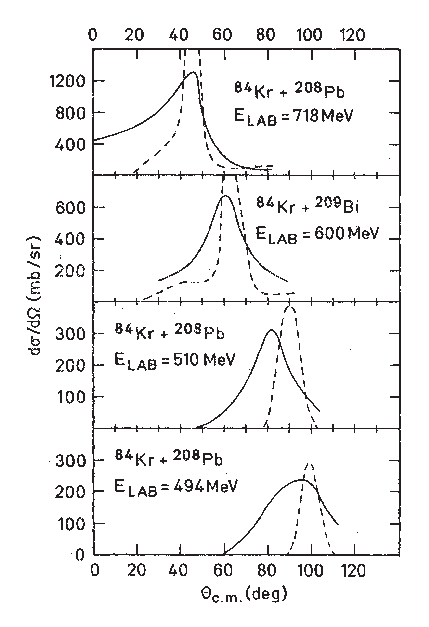
\includegraphics[clip,keepaspectratio,width=73mm]{figure/chapter4/DIC_84Kr_209Bi.eps}
      \caption{Differential cross sections for the light fragments emitted in
      $^{84}$Kr-induced reactions. The solid lines show the experimental data and the
      dashed lines show the results of the 
      Weidenm\"uller's calculation based on RMT. Taken from Ref. \cite{akw4}.}
      \label{DIC1}
    \end{minipage}
    \hspace{1.0cm}
    \begin{minipage}[t]{75mm}
      \includegraphics[clip,keepaspectratio,width=75mm]{figure/chapter4/DIC_209Bi_236Xe.eps}
      \caption{Angular distribution of fragments in the reaction of $^{136}$Xe +
      $^{209}$Bi, integrated over the energy of fragments as indicated. $\langle Z
      \rangle$ is an atomic number of fragments. The dots show the data and the
      dashed lines show the results of the calculation.
      Taken from Ref. \cite{akw4}}
      \label{DIC2}
    \end{minipage}
  \end{center}
\end{figure}
\end{document}



